\subsection{Cosmic Radiation}
\label{sec:Cosmic-Radiation-Results}
\begin{figure}[h!]
	\begin{center}
	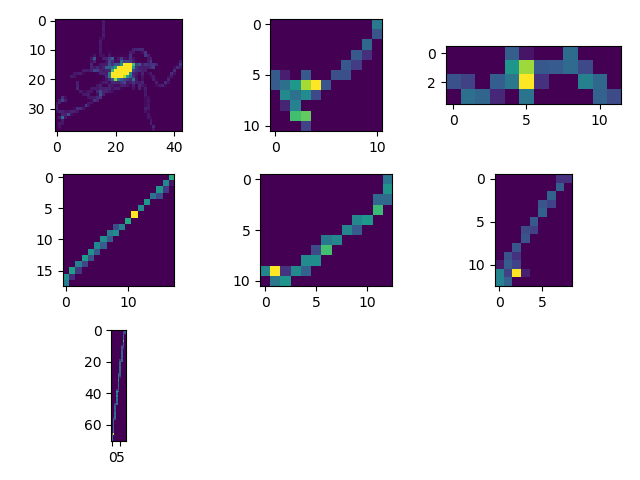
\includegraphics[width=0.8\textwidth]{figures/tracks.png}
	\caption{Tracks collected at float.}
	\label{tracks}
	\end{center}
\end{figure}

\begin{figure}
\hfill
\subfigure[LET Spectrum from data collected during the duration of the flight.]{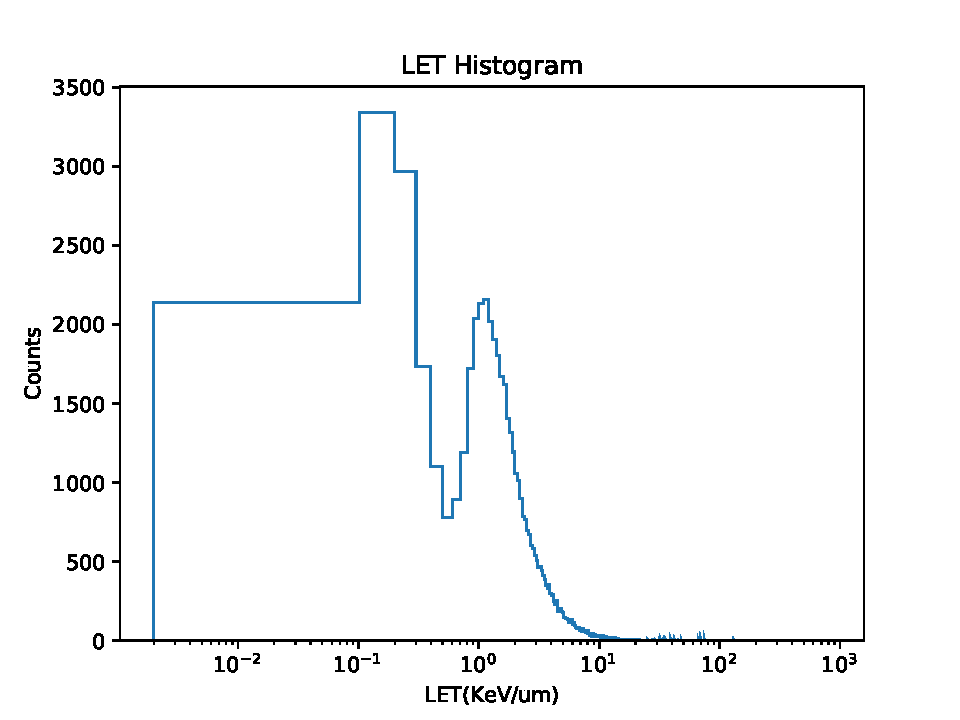
\includegraphics[width=8cm]{figures/LETSpectra2018.pdf}}
\hfill
\subfigure[LET Spectra from each cluster type.]{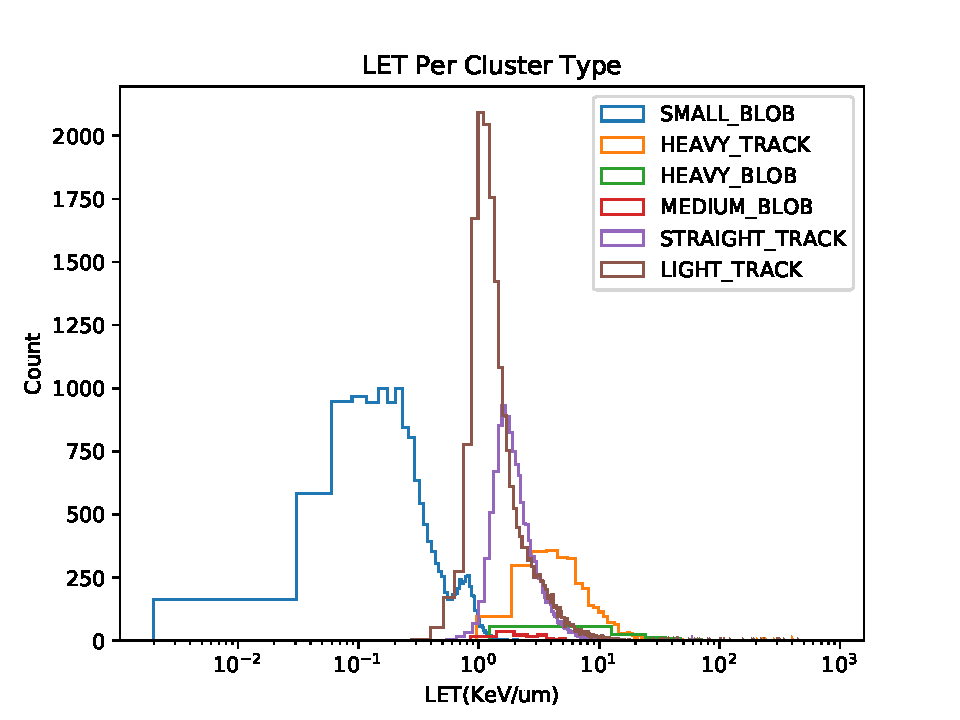
\includegraphics[width=8cm]{figures/LETSpectraPerCluster2018.pdf}}
\hfill
\caption{Title for both}
\end{figure}
